% Preambulo compartido para clases en formato beamer
\documentclass[9pt, xcolor=svgnames]{beamer}
\usepackage[utf8]{inputenc}
\usepackage[T1]{fontenc}
\usepackage[spanish,es-nodecimaldot]{babel}

\usetheme[progressbar=frametitle]{metropolis}
\metroset{sectionpage=none, subsectionpage=none}
\usepackage{appendixnumberbeamer}
\usepackage{booktabs}
\usepackage{amsmath,amssymb,bm,mathtools}
\usepackage{physics}
\usepackage{graphicx}
\usepackage{multicol}
\usepackage{tikz}
\usepackage{minted}
\usemintedstyle{tango}
\setminted{fontsize=\scriptsize, breaklines=true, linenos=true, bgcolor=LightGray!20, frame=lines}
\newminted{python}{fontsize=\scriptsize, breaklines=true, linenos=true, bgcolor=LightGray!20, frame=lines}
\usepackage{pgfplots}
\pgfplotsset{compat=1.18}
\usepackage{ragged2e}
\usepackage{xspace}
\newcommand{\themename}{\textbf{\textsc{metropolis}}\xspace}

\setbeamercolor{block title}{bg=MidnightBlue!85, fg=white}
\setbeamercolor{block body}{bg=MidnightBlue!5, fg=black}
\setbeamercolor{alerted text}{fg=Crimson}
\setbeamercolor{frametitle}{bg=MidnightBlue!10, fg=black}
\setbeamertemplate{blocks}[rounded][shadow=true]


\weektitle{04}{dinámica molecular y simulaciones de partículas}

\begin{document}

\frame{\titlepage}

\begin{frame}{Organización de la semana}
\begin{block}{Formato unificado (mismo PDF)}
La Semana 04 se divide en \textbf{Clase 1} y \textbf{Clase 2}, manteniendo el formato de semanas anteriores:
\begin{itemize}
    \item \textbf{30--45 min} de teoría breve y discusión conceptual.
    \item \textbf{75--90 min} de laboratorio guiado con Python.
\end{itemize}
\end{block}

\vspace{0.3cm}
\begin{columns}[T,onlytextwidth]
\column{0.48\textwidth}
\textbf{Clase 1}
\begin{itemize}
    \item qué es dinámica molecular y qué problemas resuelve;
    \item fuerzas interatómicas y potencial de Lennard--Jones;
    \item integración numérica: Euler, Verlet y velocity Verlet.
\end{itemize}
\column{0.48\textwidth}
\textbf{Clase 2}
\begin{itemize}
    \item flujo completo de una simulación;
    \item simulación de billar 2D y colisiones con paredes;
    \item extensiones: gravedad, colisiones entre partículas y análisis energético.
\end{itemize}
\end{columns}
\end{frame}

\section{Clase 1}

\begin{frame}[plain]
\centering
\vfill
{\Huge \bfseries Clase 1}\\[0.4cm]
{\Large Fundamentos de dinámica molecular e integración temporal}
\vfill
\end{frame}

\begin{frame}{Objetivos de la Clase 1}
\begin{itemize}
    \item Entender el vínculo entre \textbf{escala microscópica} (átomos/partículas) y \textbf{propiedades macroscópicas}.
    \item Formular el problema dinámico a partir de la segunda ley de Newton.
    \item Comparar algoritmos de integración temporal y sus errores numéricos.
    \item Implementar un primer integrador para un sistema sencillo de partículas.
\end{itemize}
\end{frame}

\begin{frame}{¿Qué es dinámica molecular?}
En dinámica molecular (MD), resolvemos numéricamente las trayectorias de muchas partículas usando:
\[
    m_i\,\ddot{\bm{x}}_i = \bm{F}_i(\bm{x}_1,\ldots,\bm{x}_N, t).
\]

\begin{itemize}
    \item Cada partícula sigue leyes clásicas de movimiento.
    \item Las fuerzas pueden incluir campos externos e interacciones entre partículas.
    \item A partir de las trayectorias, estimamos temperatura, presión, difusión y otras propiedades colectivas.
\end{itemize}

\begin{alertblock}{Idea clave}
MD traduce una ley local simple (Newton) en comportamiento colectivo complejo mediante integración iterativa en el tiempo.
\end{alertblock}
\end{frame}

\begin{frame}{Alcance y aplicaciones}
\begin{columns}[T]
\begin{column}{0.53\textwidth}
\begin{itemize}
    \item \textbf{Materiales}: defectos, elasticidad, transición de fase.
    \item \textbf{Biofísica}: plegamiento de proteínas, membranas, cápsides virales.
    \item \textbf{Fluidos}: transporte, difusión, viscosidad.
    \item \textbf{Nanoescala}: lubricación, interfaces y confinamiento.
\end{itemize}
\end{column}
\begin{column}{0.47\textwidth}
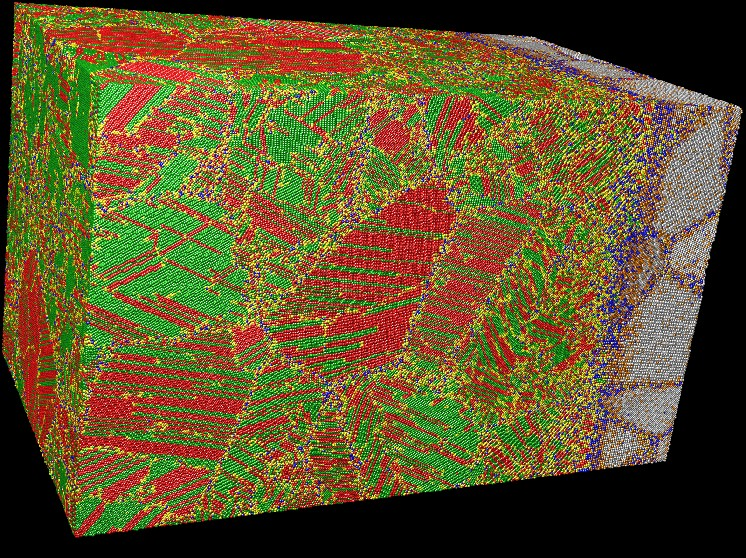
\includegraphics[width=\linewidth]{poly.jpg}
\end{column}
\end{columns}

\vspace{0.15cm}
\small Escalas típicas: \(10^3\) a \(10^7\) partículas, \(\Delta t\sim 1\) fs, simulaciones de ns a \(\mu\)s según el caso.
\end{frame}

\begin{frame}{Ejemplo de sistema biofísico}
\begin{center}
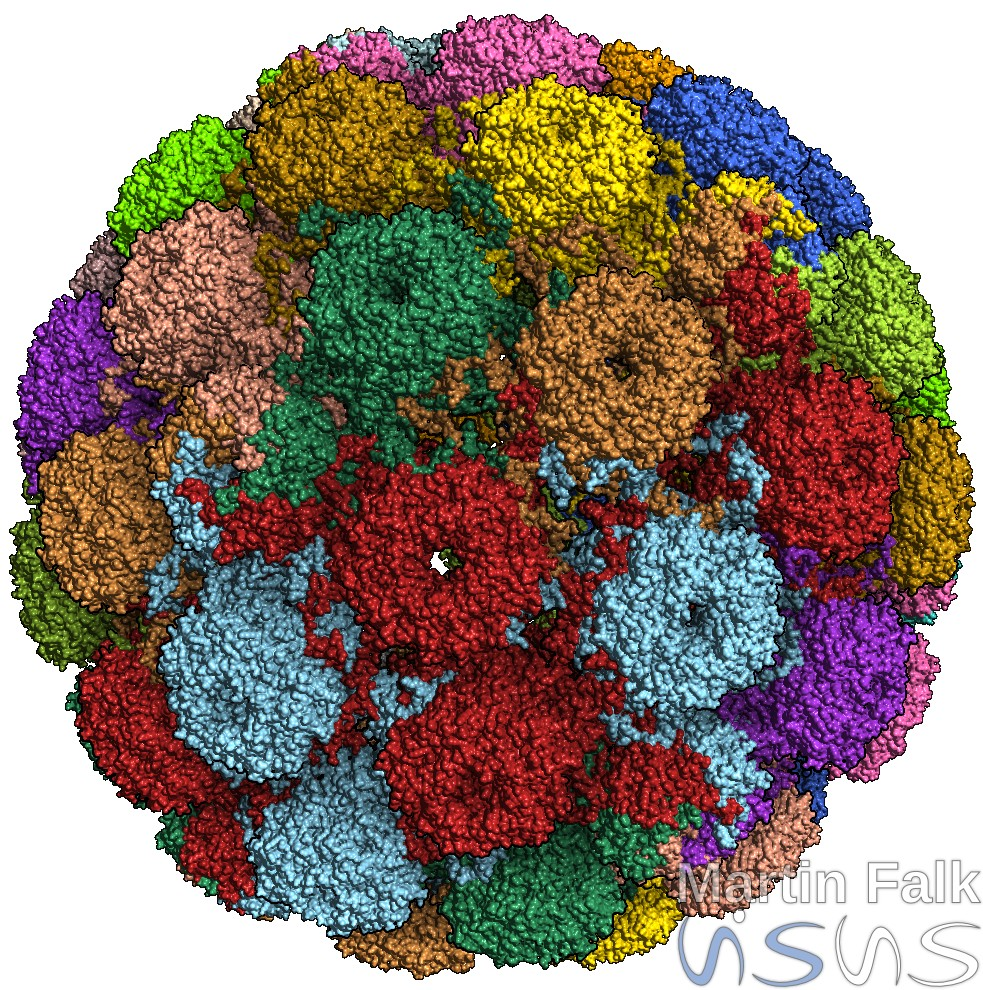
\includegraphics[width=0.62\textwidth]{virus.jpg}
\end{center}

\begin{block}{Motivación}
Modelar la envoltura de un virus permite estudiar estabilidad estructural, interacción con el entorno y respuesta ante cambios de temperatura o salinidad.
\end{block}
\end{frame}

\begin{frame}{Potencial de Lennard--Jones}
\begin{columns}
\begin{column}{0.55\textwidth}
\[
U(r) = 4\epsilon\left[\left(\frac{\sigma}{r}\right)^{12} - \left(\frac{\sigma}{r}\right)^6\right]
\]

\begin{itemize}
    \item término \(r^{-12}\): repulsión fuerte a corta distancia;
    \item término \(r^{-6}\): atracción de van der Waals;
    \item mínimo en \(r_\text{eq}=2^{1/6}\sigma\).
\end{itemize}
\end{column}
\begin{column}{0.45\textwidth}
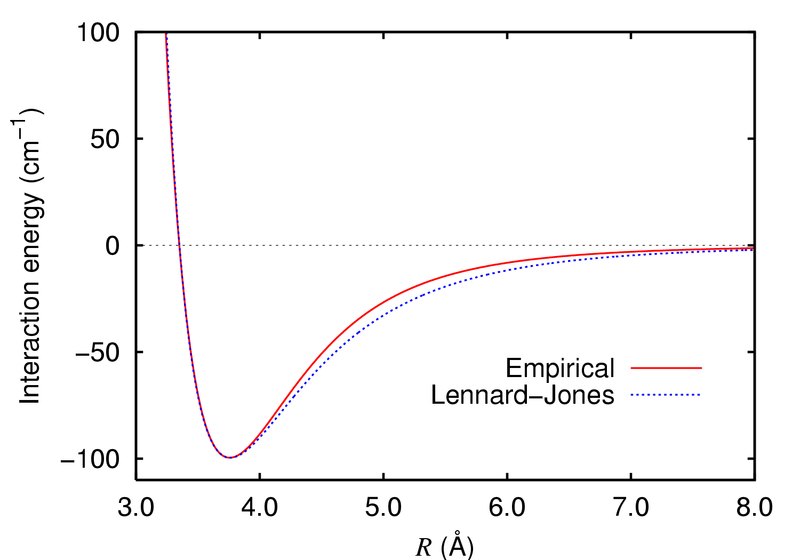
\includegraphics[width=\linewidth]{argonLJ.png}
\end{column}
\end{columns}

La fuerza radial es \(F(r)=-\dv*{U}{r}\), y en 3D se proyecta sobre el vector que une a las partículas.
\end{frame}

\begin{frame}{Flujo mínimo de un programa de MD}
\begin{enumerate}
    \item Definir posiciones iniciales, velocidades y parámetros físicos.
    \item Calcular fuerzas a partir del potencial elegido.
    \item Integrar posiciones/velocidades un paso \(\Delta t\).
    \item Medir observables (energía, temperatura, presión, difusión).
    \item Repetir por muchos pasos y analizar la evolución temporal.
\end{enumerate}

\begin{block}{Buenas prácticas}
Separar el código en funciones \texttt{fuerzas()}, \texttt{integrador()}, \texttt{observables()} mejora claridad y reutilización.
\end{block}
\end{frame}

\begin{frame}{Métodos de integración}
\small
\textbf{Euler explícito}
\[
\bm{x}_{n+1}=\bm{x}_n+\bm{v}_n\Delta t,\qquad
\bm{v}_{n+1}=\bm{v}_n+\bm{a}_n\Delta t
\]
Simple y barato, pero con deriva energética importante para simulaciones largas.

\vspace{0.2cm}
\textbf{Verlet}
\[
\bm{x}_{n+1}=2\bm{x}_n-\bm{x}_{n-1}+\bm{a}_n(\Delta t)^2
\]
Mejor estabilidad; no usa velocidad explícita en el paso principal.

\vspace{0.2cm}
\textbf{Velocity Verlet}
\[
\bm{x}_{n+1}=\bm{x}_n+\bm{v}_n\Delta t+\frac12\bm{a}_n(\Delta t)^2
\]
\[
\bm{v}_{n+1}=\bm{v}_n+\frac12(\bm{a}_n+\bm{a}_{n+1})\Delta t
\]
Estándar en muchos códigos de MD por su equilibrio entre precisión y costo.
\end{frame}

\begin{frame}[fragile]{Código ejemplo: Euler para partícula libre 2D}
\inputminted{python}{md_euler.py}
\end{frame}

\begin{frame}[fragile]{Código ejemplo: paso velocity Verlet (Lennard--Jones)}
\inputminted[firstline=1,lastline=55]{python}{md_velocity_verlet.py}
\end{frame}

\begin{frame}{Cierre Clase 1}
\begin{itemize}
    \item Dinámica molecular = integración repetida de Newton + modelo de fuerzas.
    \item La elección del integrador afecta estabilidad, precisión y costo computacional.
    \item Antes de escalar el sistema, conviene validar con ejemplos pequeños y chequeo de energía.
\end{itemize}
\end{frame}

\section{Clase 2}

\begin{frame}[plain]
\centering
\vfill
{\Huge \bfseries Clase 2}\\[0.4cm]
{\Large Taller guiado: billar 2D, colisiones y extensiones físicas}
\vfill
\end{frame}

\begin{frame}{Objetivos de la Clase 2}
\begin{itemize}
    \item Implementar una simulación 2D de partículas en caja con rebotes en paredes.
    \item Incorporar aceleración constante (gravedad) con velocity Verlet.
    \item Proponer colisiones entre partículas y monitorear energía cinética total.
    \item Relacionar decisiones numéricas (\(\Delta t\), condición de colisión) con resultados físicos.
\end{itemize}
\end{frame}

\begin{frame}{Sistema de billar bidimensional}
\begin{columns}
\begin{column}{0.52\textwidth}
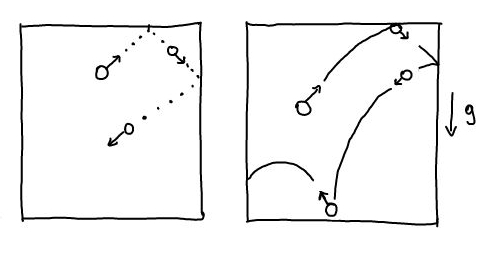
\includegraphics[width=\linewidth]{billares.jpg}
\end{column}
\begin{column}{0.48\textwidth}
\begin{block}{Reglas de rebote en caja}\small
\begin{itemize}
    \item choque con pared vertical: \(v_x\to -v_x\)
    \item choque con pared horizontal: \(v_y\to -v_y\)
\end{itemize}
\end{block}

\begin{itemize}
    \item Sin fuerzas, la rapidez de cada partícula se conserva.
    \item Con gravedad, la energía potencial intercambia con la cinética.
\end{itemize}
\end{column}
\end{columns}
\end{frame}

\begin{frame}{De pseudocódigo a implementación}
\small
\begin{enumerate}
    \item Inicializar \(\bm{x}_i,\bm{v}_i\) para cada partícula dentro de la caja.
    \item Actualizar posiciones y velocidades en cada \(\Delta t\).
    \item Corregir rebotes cuando una coordenada sale de \([0,L]\).
    \item Registrar trayectorias y magnitudes globales (energía, número de choques).
\end{enumerate}

\begin{alertblock}{Pregunta de modelamiento}
¿Qué cambia al resolver choques partícula--partícula de forma determinista (conservando momento) versus usar una regla aleatoria simple?
\end{alertblock}
\end{frame}

\begin{frame}[fragile]{Código ejemplo: billar 2D con rebotes y gravedad}
\inputminted{python}{billiard_2d.py}
\end{frame}

\begin{frame}[fragile]{Extensión sugerida: detector simple de colisión}
\inputminted[firstline=57,lastline=91]{python}{md_velocity_verlet.py}
\end{frame}

\begin{frame}{Actividades propuestas (90 min)}
\begin{enumerate}
    \item \textbf{Base}: simular dos partículas sin aceleración (Euler).
    \item \textbf{Extensión A}: incluir gravedad y comparar Euler vs velocity Verlet.
    \item \textbf{Extensión B}: agregar colisiones partícula--partícula con radio efectivo.
    \item \textbf{Análisis}: graficar energía total y discutir estabilidad numérica al variar \(\Delta t\).
\end{enumerate}

\begin{block}{Entregable sugerido}
Notebook o script con gráficos de trayectorias + breve discusión sobre precisión, costo y comportamiento físico observado.
\end{block}
\end{frame}

\begin{frame}{Cierre de la semana}
\begin{itemize}
    \item MD conecta ecuaciones locales con fenómenos colectivos emergentes.
    \item El diseño del algoritmo (integrador, detección de colisiones, paso temporal) es parte del modelo físico.
    \item La Semana 04 deja una base para escalar a más partículas y estudiar sistemas reales.
\end{itemize}

\vspace{0.2cm}
\centering
\textbf{Próximo paso recomendado:} implementar listas de vecinos para acelerar el cálculo de fuerzas.
\end{frame}

\end{document}
